% vim: ft=tex
\chapter{Approach}
This chapter describes the approach taken by the students to fulfill the
requirements. Possible variants as well as the final choices are explained here.

\section{Overview}
% TODO * testing env, specs (~150 -> ~900)
% TODO * actor layer: new actors, fed sockets, encryption, codecs (moved down and added authentication feature), messageauthenticator
% TODO * messaging layer: new handlers, new protocols (FCP, BSP), new messages, "@node",
% TODO * engine layer: new engines (Upstream, Downstream, BStar), Host extensions (#find_node), CSPMethods, MessageAuthentication, SupernodeSelector, SubnodesSelector, Domain::Model::Node


\section{Testing}
This section describes the test methods used to check units, the integration of
multiple components, as well as the behavior of new contributions across the
entire framework.  All test results are described in \autoref{ch:res}.

The following subsections describe in detail how testing is performed.

\subsection{Unit tests}
To ensure the correctness of the implementations, unit tests are written using
RSpec. 100\% coverage of the students' contributions can be achieved by
adhering to \gls{TDD}, or more specifically, \gls{BDD}. RSpec offers itself as
a very valuable testing tool providing very expressive assertion and mocking
facilities, as well as more advanced features such as testing spies which have
proven to be a perfect use case for Ruby's dynamic binding (a.k.a \emph{duck typing}
\footnote{\url{https://en.wikipedia.org/wiki/Duck_typing}}).

Naturally, this also simplifies refactoring the code without the risk of
breaking functionality unnoticed. Unit tests reside under the \sh{spec}
directory of Roadster's code base.

% TODO RSpec extension
% TODO typical test example
% TODO speccing only public methods and side effects of private methods

\subsection{Integration tests}
Integration tests verify the interaction between the individual components.
To test new core functionality like federation, high availability, and persistence
synchronization, integration tests have been written.

In order to test the failover or synchronization functionality, individual processes
can simply be killed and restarted later if the scenario defines this.


\subsection{System tests}
System tests are designed to test the application under close-to-reality
conditions, treating the application as a black box: On a certain input, it is
supposed to react with a certain output. The internal mechanisms to produce said
output and reach a certain state are insignificant.

% TODO how to test persistence synchronization

\paragraph{Manual} At times when developing a feature, manual testing can give
useful insights, especially when trouble shooting. Running Roadster manually in
foreground within a terminal session helps with that.  When, for example,
developing a new inter-node protocol, running multiple nodes simultaneously
becomes a necessity. Although on the same development machine, this can be
simulated by starting them as different process groups. Through the
configuration, each Roadster instance is given a different set of endpoints,
e.g. different TCP ports or Unix domain sockets. This is possible and feasible
since \zmq completely abstracts the transport away and thus really doesn't
matter if other Roadster instances are running locally or remotely.

\paragraph{Automated} To create an more realistic environment including real
network conditions, a more lower level approach is taken. Stronger isolation
between Roadster instances can be achieved using software containers. Network
virtualization can be used to induce latency and packet loss to simulate the
properties of a congested network.
Docker and Mininet together provide all of the required functionality.

When a feature depends on external sensor data from a field device (e.g. a \gls{PLC}),
a fake adapter is used. It continually fakes the actions of a fictional robot.

\begin{description}
	\item [Docker:]\hfill\\
		Docker is a container software that makes use of the
		\emph{cgroups}\footnote{\url{https://en.wikipedia.org/wiki/Cgroups}}
		feature of the Linux kernel, which allows the isolation of
		collections of processes. This includes isolation of CPU,
		memory, and I/O usage, as well as process ID and network
		namespaces.

		Docker also provides a programmable way to start with a clean
		state at the beginning of every run of the test suites. All
		state changes and file system modifications are discarded after
		the container is stopped.

	\item [Mininet:]\hfill\\
		Mininet allows creating virtual networks instantaneously.
		Like Docker, it also relies on \emph{cgroups}
		and network namespaces to efficiently run multiple \glspl{VM}
		sharing the same kernel, and provide isolation. These very same
		primitives are used by Docker itself.

		Network infrastructure such as packet switching hardware and
		network links can be modeled in Mininet, including the
		simulation of link quality issues such as induced latency and
		packet loss.

	\item [Fake adapter:]\hfill\\
		A fake implementation of a fictional \gls{PLC}, namely a robot
		that that changes its position randomly in a 2D coordinate
		system serves the purpose of getting external sensor data.
		Using Roadster's guards it will also generate cases as soon as
		it moves out of a predefined, virtual bounding box. This robot
		is implemented using about 15 lines of Ruby code and is part of
		the example application provided by mindclue GmbH.
\end{description}

The system test results from each construction iteration can be found in \autoref{ch:res}.


\subsection{Continous integration}
\Gls{CI} helps prevent problems when integrating big chunks of code changes,
also known as \emph{integration hell}. A new CI build is triggered upon each
push of changes to the repository using a predefined build script.

\paragraph{GitLab CI} Due to the fact that Roadster's GitHub repository is private, online \gls{CI}
services such as \emph{Travis~CI}\footnote{\url{https://travis-ci.com/}, requires payment after the
first 100 builds} cannot be used without payment. Fortunately,
GitLab\footnote{\url{https://about.gitlab.com}} is a free, open-source GitHub-like development collaboration software and includes CI functionality. It can be installed on private infrastructure, such as the
\gls{VM} provided by HSR, where it has been installed and configured.

\paragraph{Auto triggering} Every push of changes to Roadster or the example application triggers the CI
solution set up on the HSR VM. It then installs Roadster's dependencies, the Roadster
framework itself, the example application, and then runs all of Roadster's test
suites. This is useful to get informed proactively when something breaks.

\subsubsection{Documentation build}
It is deemed bad practice to keep generated files in a Git
repository. Having an additional file to commit is tedious and if done
frequently, it can bloat the repository's commit history since Git treats PDF
files as binary files, and thus cannot use efficient algorithms to work out the
differences only.

This is why compiling the TeX sources for this document is also done reactively
via a pipeline configured on GitLab CI. The resulting artifact, a PDF file, is
then automatically uploaded to Git as a file associated with a newly created
public release. This is done via GitHub's webservice API for managing
releases.\footnote{\url{https://developer.github.com/v3/repos/releases/}}


\subsubsection{Docker container}
To provide a clean test environment for every CI build, a Docker container is used.
It prepares the container with all necessary components before every build
which then runs all test suites. The components include:

\begin{itemize}
	\item Mininet
	\item Ruby
	\item Python
	\item The most recent development version of Roadster (of the appropriate branch)
\end{itemize}

The system tests are run on the GitLab server after each construction
iteration. To do so, the Python scripts set up a virtual network and then start
the appropriate Roadster instances. Some features require a link to fail or a
node to fail, which can be achieved at arbitrary times through Mininet commands or
simply kiling Roadster instances wherever needed. The generated log data is
evaluated later to verify that the behavior for each defined feature is
correct.


\subsubsection{Test scenarios}
Test scenarios are deduced from the features specified in \autoref{ch:reqs}.
They contain configurations for Mininet and the particular Roadster nodes.
The procedure of each scenario is modeled in feature step files. This subsection
describes the implementation and general structure of the test scenarios in detail.


Every run of the system tests is based on the current versions of

\begin{itemize}
	\item The Roadster framework itself
	\item The example application
\end{itemize}

In case the current development is taking place in a feature branch, the same
branch is tried to be checked out in both test working copies. For example to
test a new feature like encryption, it is developed in a feature branch called
\emph{encryption} in Roadster's repository. Because the example application
will need modifications as well (such as the knowledge of public keys for each
node in a federation), it those changes are implemented in a feature branch of
the same name.

A shell script creates the appropriate configuration files (fixtures) before
each test scenario is run and ensures that a directory for each Roadster
instance exists where log data is stored during the run.

Mininet is a Python library. To interactively use Mininet, it makes sense to
implement all system test code in Python. This allows taking influence on the
virtual network and on particular hosts within that network at any time. To
parse and evaluate the features written in the Cucumber format, the BDD
framework Behave\footnote{\url{http://pythonhosted.org/behave/}} is used.

\subsubsection{Directory structure}

The directory structure used within the Docker container is illustrated
in~\autoref{lst:testing:docker:directory-structure}.

\begin{listing}
	\begin{minted}[bgcolor=bg]{Shell}
/tmp/
|-- roadster
|   |-- ci
|   |   |-- run_system_tests.sh
|   |   `-- run_unit_tests.sh
|   `-- features
|       |-- autonomy.feature
|       |-- environment.py
|       |-- ...
|       |-- steps
|       |   |-- autonomy.py
|       |   |-- behave_util.py
|       |   `-- ...
|       |-- support
|       |   |-- conf.root.primary.rb
|       |   |-- federation.rb
|       |   `-- ...
`-- projects
	`-- ba-roadster-app
		|-- conf.root.primary.rb
		|-- data.root.primary
		|   |-- eventjournal.tct
		|   `-- parameters.tch
		|-- lib
			|-- domain
			|   |-- federation.rb
			|   `-- ...
			`-- ...
	\end{minted}
	\caption{Directory structure of system tests within Docker container}
	\label{lst:testing:docker:directory-structure}
\end{listing}

\subsubsection{Roadster federation topology}
The federation used for system tests is build as follows:
\begin{figure}[]
	\center
	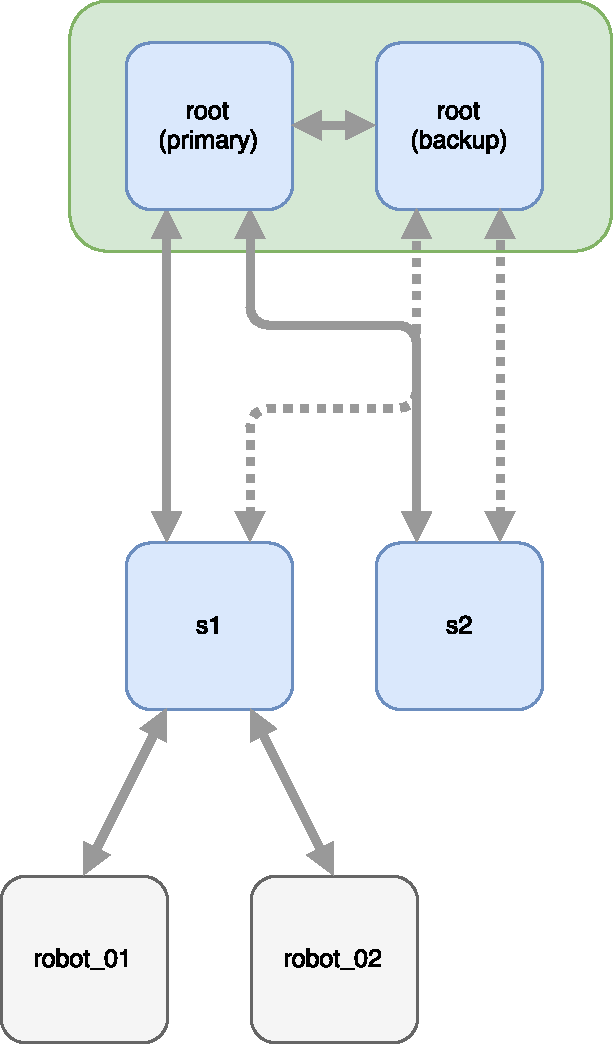
\includegraphics[width=0.5\textwidth]{img/logical_federation_setup.pdf}
	\caption{Logical federation topology used in system tests}
	\label{lst:testing:topo:logic}
\end{figure}

The root node is a HA cluster, which acts as such when appropriate according to
the feature being tested. At other times, only its primary node is active and
thus acts as a non-HA supernode of sN1 and sN2. The naming scheme is enforced
by Mininet and thus somehow clunky and cryptic.

The configuration also dictates that there are two simulated robots running on
subnode sN1, which continually update sensor data in the DIM and create new
cases due to their nature of virtually moving around randomly and thus trying
to escape the bounding box.

Subnode sN2 merely acts as a listener and is not directly supervising any field
devices.

\subsubsection{Virtual network plan}
\begin{figure}[]
	\center
	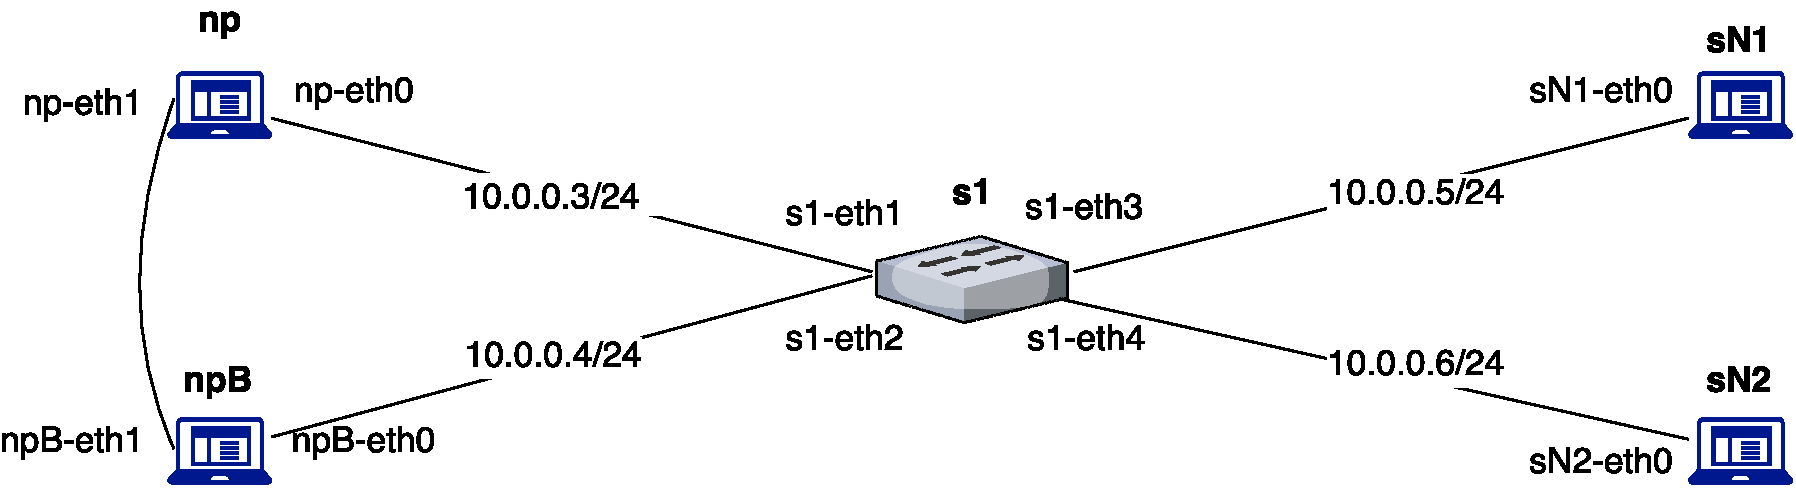
\includegraphics[width=\textwidth]{img/physical_network_mininet.pdf}
	\caption{Physical federation topology used in system tests}
	\label{lst:testing:topo:logic}
\end{figure}

All nodes are attached to an \gls{ovs} instance which allows them communicate with each
other via the TCP/IP transport. In addition to this star topology, there is an
additional, dedicated link between the two HA peers which form the root HA
cluster.

%----------------------------------------------------------------------------

\section{Port to new \zmq library}\label{sec:approach:port}
One of the first changes to Roadster's codebase is porting to a new \zmq
library. This makes sense for the following reasons:

\begin{itemize}
\item To exclude possible failures from faults in the unmaintained ffi-rzmq\footnote{\url{https://github.com/chuckremes/ffi-rzmq}} library.
\item Encryption is needed later anyway, which is not supported by the currently used library.
\item All other tasks involve \zmq communication anyway.
\end{itemize}

There is currently only a single Ruby library that is maintained, supports
encryption, and freely available, which is \gls{cztop}. Technically it's a
binding for the \gls{czmq} library, which is the modern and recommended way of
using \zmq. More info about CZMQ can be found in \autoref{ch:zmq}.

As stated in the Task Description already, Roadster's event loop makes use of
the \zmq options \sh{ZMQ_FD} and \sh{ZMQ_EVENTS}. Getters for these had to be
added to in CZTop, which was a matter of minutes.

\subsection{Actual port}
Due to Roadster's software architecture which cleanly separates different concerns, code that actually made use
of the ffi-rzmq library directly was located in a single file. The following
things needed to be done:

\begin{itemize}
\item Tell Ruby to load CZTop instead of ffi-rzmq.
\item Remove code to manually send and receive the parts of multi-part messages. This has been simplified
in CZMQ and thus is a single method call using CZTop.
\item Remove error checking code. CZTop always checks error codes, and raises
an appropriate exception if needed.
\item Simplify code that reads option values such as \sh{ZMQ_FD} and \sh{ZMQ_EVENTS}.
\item Rewrite library calls to use CZTop instead of ffi-rzmq.
\end{itemize}

This was about an hour's work.

\section{Getting familiar with Roadster}


\section{Prototypes}
As a way of getting familiar with the Roadster code base, as well as to prove
the concepts worked out during the early elaboration phase, two prototypes have
been programmed during the later elaboration phase of this thesis. The client
and main author of Roadster was immensely helpful by giving an introduction to
the code base early on.  Although quite overwhelming, the first impression was
that the code is clean, makes good use of abstractions and has loosely coupled
classes.

% TODO: describe approach of getting more familiar with Roadster, during prototyping

The two prototypes, namely the inter-node communication and the high availability
mechanism, have been developed with "cheap, quick, and dirty" in mind. The
approach to these two prototypes are described briefly in the next sections.


\subsection{Inter-node communication}
The idea of this prototype was to achieve rudimentary communication between two
Roadster nodes.
% TODO general idea of prototype

To do so, new actors need to be added for the communication with neighboring nodes of the
federation.  Since COMM actors are used to communicate with systems outside of
a node, the new actors are:
\begin{description}
\item [COMM.UPSTREAM]\hfill\\
This actor is responsible for communication with the direct supernode.
\item [COMM.DOWNSTREAM]\hfill\\
This actor is responsible for communication with direct subnodes.
\end{description}


% TODO: translate, nicht sicher ob der zusammenhang korrekt ist
Um Nachrichten über die neuen Actors zu senden, wurde ein FCP Protokol
erstellt. Dabei wurde im Prototyp ein einfaches Hello verschickt.
Das FCP Protokol wurde nach der Entwicklung der Prototypen dazu verwendet um Nachrichten 
in der Federation von Punkt A zu Punkt B zu routen. In erster Linie dient es für Routing aber es wird auch für geroutete
Ping \& Pong Nachrichten verwendet. Die Ping \& Pong Nachrichten
dienen zur Überwachung der Erreichbarkeit der Subnodes und des Supernodes.
Weiteres zum Protokol im Kapitel Message routing.
% TODO: describe in layers
% TODO: FCP::API, FCP::API::Hello message


% FIXME: this is too detailed
\paragraph{Background info: Servers and clients in \zmq}
Usually in network programming, the server is the one performing the
\cpp{bind()} operation and the client is the one performing the \cpp{connect()}
operation. This restriction does not hold true in \zmq. Since \zmq completely
abstracts the connection handling away, the order in which these two operations
happen is insignificant. In case the other side has not bound its socket
yet, \zmq will just retry establishing a connection if the last attempt failed,
by default every 100 milliseconds. This means that it is a free choice as to which socket
performs what action. Each socket type merely has default action for the case
it is initialized with a given endpoint.

\paragraph{Intuitive server and client roles}
% FIXME: needed?
Even though the client of a Roadster federation (if it is not a standalone
Roadster installation) logically resides above the root node, within a Roadster
federation, the choice has been made to assign the roles more intuitively. A
supernode's DOWNSTREAM actor will \cpp{bind()} its socket, and a subnode's
UPSTREAM actor will \cpp{connect()} to its supernode. This is consistent
with the server role mentioned in \autoref{sec:scope:csp}, and will later be
relevant for transport security as well (see \autoref{sec:approach:encryption}).

Of course, in a multi level hierarchy with three or more levels, the
intermediate nodes would act as servers of their subnodes, and as clients of
their supernodes. This translates to: They are running both an UPSTREAM and a DOWNSTREAM
actor.

As described in \autoref{sec:scope:csp}, there are three distinct message flows
in the \gls{CSP}. The same applies to inter-node DIM synchronization. A
supernode with multiple subnodes will act as the server in CSP terminology.

\begin{description}
	\item [UPSTREAM:]
		This actor's responsibilities are providing a
		communication interface to the supernode, if any. To do so, it
		creates and \cpp{connect()}s three different sockets to fulfill
		its complete set of tasks. These three sockets are of type
		DEALER, PUSH, and SUB.

	\item [DOWNSTREAM:]
		To fulfill its part of the CSP, this actor creates
		and \cpp{bind()}s three sockets of type ROUTER, PULL, and PUB.
\end{description}


\subsection{High availability}
% TODO: standalone tests

%----------------------------------------------------------------------------
\section{Federation}\label{sec:approach:federation}
% TODO: big picture
A Roadster federation is illustrated in \autoref{fig:federation}. Adding federation
functionality to Roadster involves the following aspects:
\begin{itemize}
	\item A \gls{DSL} to be able to define a federation (including the role of each node)
	\item Message routing
	\item Heartbeating
	\item DIM synchronization
\end{itemize}

\begin{figure}[]
	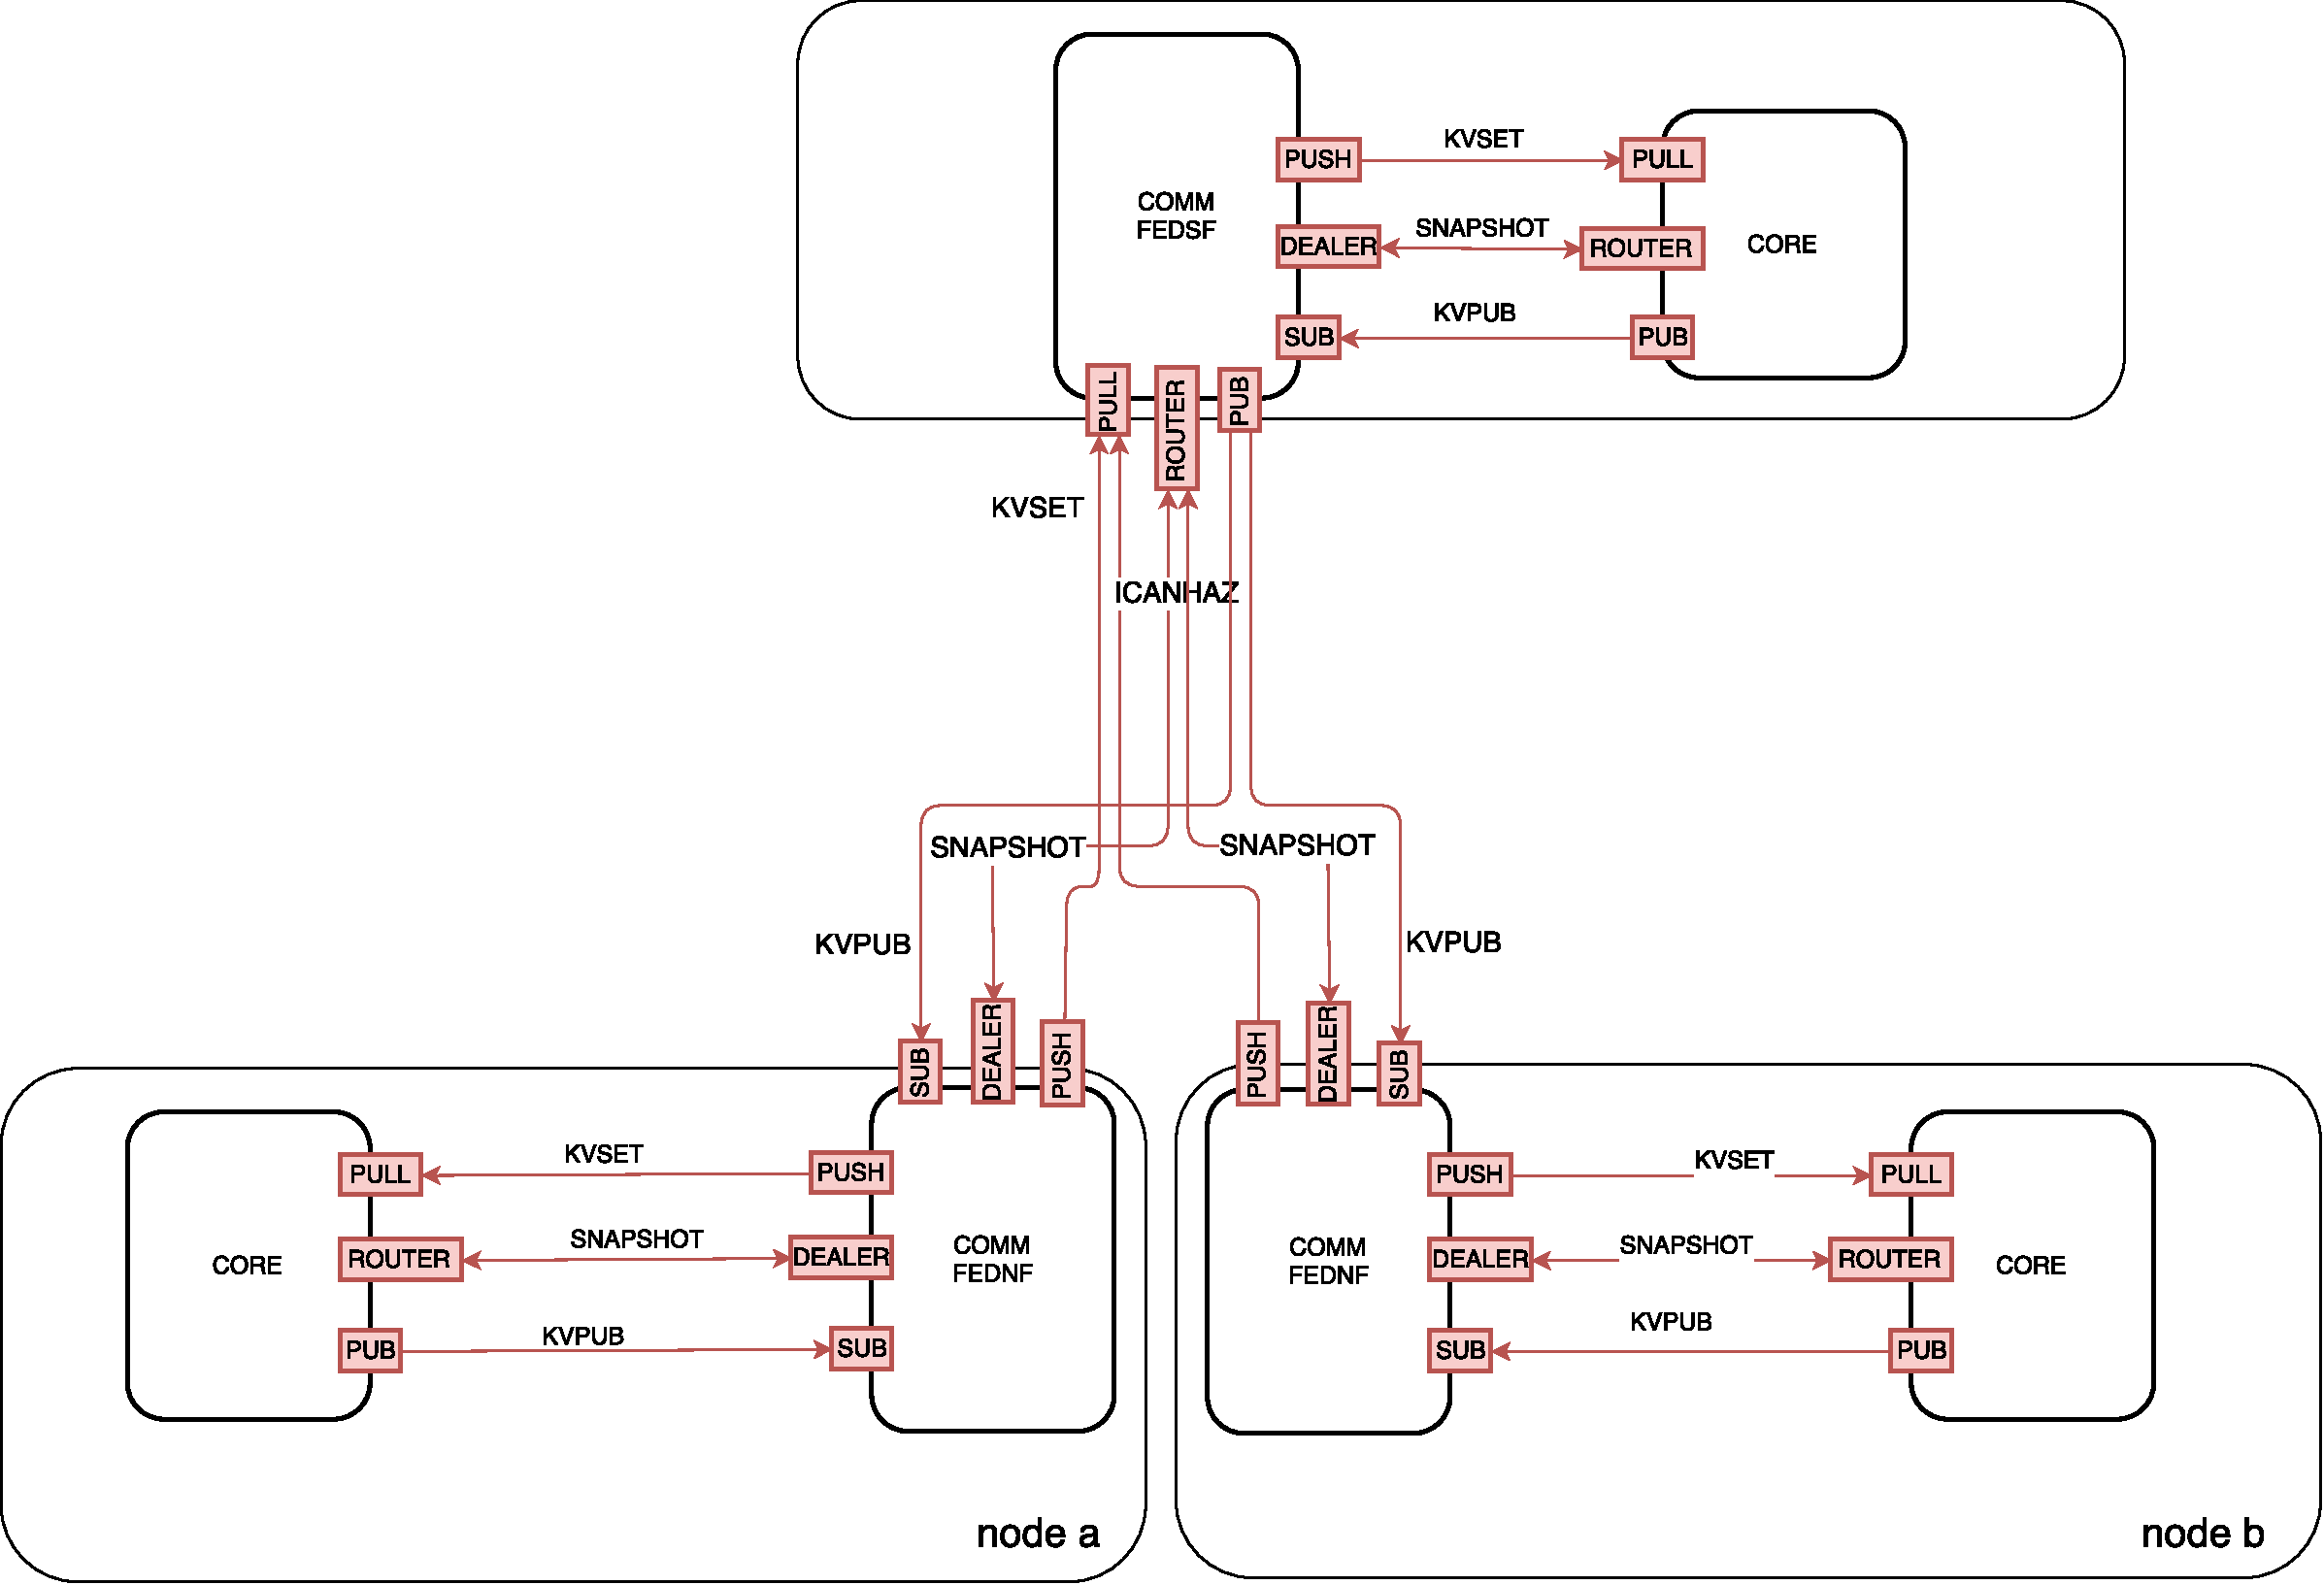
\includegraphics[width=\textwidth]{img/federation_protocol.pdf}
	\caption{Federation between a supernode and two subnodes}
	\label{fig:federation}
\end{figure}

\subsection{Federation definition}
% TODO: topolofy_conf.rb rename to federation.rb?
The federation topology has to be defined somewhere. This can be done using a
\gls{DSL} and then put into a static file (e.g. \sh{topology_conf.rb}) shared
on all nodes of a Roadster federation. Each actor could then read the file at
startup, just like it is done for other configuration pieces of a Roadster node.
\autoref{lst:dsl:topo:no-ha} shows how such a configuration snippet might look.

% TODO: FIXME text isn't correct anymore
To let the actors of a node know which node they belong to, an additoinal line
has to be added to the specific configuration file (\sh{conf.rb}), e.g.
% FIXME: root node could be called nodes.northpole (avoids ambiguity with the
% root element of the DIM)
\rb{conf.system_id = "nodes.root"}. Using that information, the topology
created using the DSL can be walked like a tree to find the correct node and
important information like its neighbor nodes.

A HA node pair could be one DIM object which has one name but two IP addresses
(primary and backup, in that order). Direct subnodes can use that information
to connect to the correct supernode during normal operation and also
when the primary node is unavailable. The respective DSL snippet is shown in
\autoref{lst:dsl:topo:with-ha}.

Not every node in a federation has the same role: Some are only connected with other
nodes, some directly communicate with field devices. To define different node roles, a
syntax as shown in \autoref{lst:dsl:topo:with-roles} is possible.

An entirely different approach would solve this problem using a hierarchical
property list format, e.g. ZPL.\footnote{\url{https://rfc.zeromq.org/spec:4/ZPL}}
A definite decision has yet to be made.

% TODO node-specific config file

\begin{listing}
	% TODO: update to declarative form
	\begin{minted}[bgcolor=bg]{Ruby}
module Conf::Federation
  def self.conf
    proc do
      primary_endpoints \
        router: 'tcp://0.0.0.0:20000',
        pull:   'tcp://0.0.0.0:20001',
        pub:    'tcp://0.0.0.0:20002',
        ha_pub: 'tcp://0.0.0.0:20003'

      adapters do
        adapter :foobar do
          # config for 'foobar' adapter and its peers
        end
      end

      node :s1 do
        primary_public_key '4V]RsRk}.=dcAwNkXH0Tj[<jVhyV7l!-Hb}t=YQ$'.b

        adapters do |s1_node|

          adapter :simu do
            label           'SIMU'
            desc            'Process simulation adapter'
            adapter_class   Roadster::Adapters::Simulation

            peer :robot_controller_01 do
              label 'robot_01'
              uri   ''
            end

            peer :robot_controller_02 do
              label 'robot_02'
              uri   ''
            end
          end
        end

        objects do |s1_node|
          robot :robot_01 do
            label_i18n  de: 'Mein schicker roboter nummer 1',
                        en: 'My fancy robot number 1'
          end
          s1_node.objects.robot_01.reference_peer s1_node.adapters.simu.robot_controller_01

          robot :robot_02 do
            label_i18n  de: 'Mein schicker roboter nummer 2',
                        en: 'My fancy robot number 2'
          end
          s1_node.objects.robot_02.reference_peer s1_node.adapters.simu.robot_controller_02
        end
      end
    end
  end
end
	\end{minted}
	\caption{Federation DSL example without HA}
	\label{lst:dsl:topo:no-ha}
\end{listing}

\begin{listing}
	\begin{minted}[bgcolor=bg]{Ruby}
module Conf::Federation
  def self.conf
    proc do
      primary_endpoints \
        router: 'tcp://0.0.0.0:20000',
        pull:   'tcp://0.0.0.0:20001',
        pub:    'tcp://0.0.0.0:20002',
        ha_pub: 'tcp://0.0.0.0:20003'

      backup_endpoints \
        router: 'tcp://0.0.0.0:20010',
        pull:   'tcp://0.0.0.0:20011',
        pub:    'tcp://0.0.0.0:20012',
        ha_pub: 'tcp://0.0.0.0:20013'

      adapters do
        # telnet server for client systems (fake OPC-UA HA interface)
        adapter :telnet do
          label           'Telnet'
          desc            'Telnet Server'
          adapter_class   Roadster::Adapters::TelnetServer

          peer :server do
            label   'LTA'
            desc    'LTA'
            uri     "tcp://0.0.0.0:#{Roadster.conf.telnet_server_port}"
          end
        end
      end

      node :s1 do
        # [...]
      end
    end
  end
end
	\end{minted}
	\caption{Fedreation DSL example with HA}
	\label{lst:dsl:topo:with-ha}
\end{listing}

% ############
% # within ba-roadster-app's lib/domain/domain.rb file:
% #
\begin{listing}
	\begin{minted}[bgcolor=bg]{Ruby}
module Roadster
  module Domain::Model

    build do
      label 'BA Roadster App'
      desc  'Sample application for P. Wenger and M. Schuler at HSR.'

      load_conf ::Conf::Federation
      load_conf ::Conf::AccessControl
      load_conf ::Conf::Navigation
    end

  end # Domain::Model
end # Roadster
	\end{minted}
	\caption{Federation DSL example with HA and roles}
	\label{lst:dsl:topo:with-roles}
\end{listing}


\subsection{Message routing}
Messages need to be sent from an actor on one node to an actor on another node.
The best place to put this logic is the CORE actor which already does this for
messages exchanged within a node. It needs to be extended to know about nodes
and their actors, not only actors on the current node. Then messages can be
passed around hop-by-hop.

In case a message is sent in \emph{Dialog} mode, this implicates Russian doll
routing: At every hop, a new dialog is started which expects an immediate
response, which will subsequently be passed back and complete the open dialogs.

% TODO: goes hand in hand with cryptographic signing, needed for end-to-end security anyway since on transport level it's only secure hop by hop

% TODO: Thoughts
% ==============
%
% * sender is origin node
%   - as of now, sender is always last hop
% * receiver is destination node
%   - as of now, receiver is always next hop
% * stateless routing (not actually matrjoshka-like)
% * message BLOB itself stays exactly the same from source to destination node
% * message envelopes are not serialized anymore (was a smell anyway, since they were replaced on the receiving side)
% * Core looks up next hop, and only next hop
%   - if next hop can't be determined, discard message
% * transport options
%   - a hash, modified on each hop
%   - serialized as ZMTP metadata
%     - as additional ZMQ frame (always present, even intra-node communication)
%   - contains:
%     - next hop node name so ROUTER socket in Downstream knows where to send to
%     - (no other trusted data, or data that survives longer than one hop, as it's not signed)
%
% TODO: stateless routing
% TODO: TTL not needed, because trees are acyclic
% TODO: security tag (why not hash node path)
% TODO: ZMTP metadata ABNF

% TODO: why not ZMTP 3.0 heartbeating:
% 1) ZMTP 3.1 is in DRAFT state
% 2) silent disconnect, not useful
% 3) intended for detection of stale TCP connections/blocked processes
% 4) only between two sockets
%
% application heartbeating is better:
% `Downstream->Core->Downstream->Upstream->Core->Upstream->Downstream`
% (includes both Cores)


\subsubsection{Example}
When a user of the root node's web UI wants to change a value on a field device
connected to the root node's subordinate node, a command is sent from the
browser to the web UI's COMM actor. From there it is sent via the CORE actor out
on the DOWNSTREAM actor to the subordinate node. There it is routed
via the CORE actor to the correct COMM actor, where the command can actually be
executed on the field device.

\subsubsection{Heartbeating}
% TODO supernode pings subnodes, subnodes send back pong
* ping/pong with sequence number to match pongs to pings
  why not dialog? => ping is one-to-many via PUB socket


\subsection{DIM synchronization}
The DIM has to be replicated across a hierarchical federation of nodes.
% TODO: more/better

The new actors' responsibility is the inter-node synchronization of the DIM,
similarly to what is happening in the existing \gls{CSP} within a single node.
To do so, they simply subscribe to DIM updates within a node just like any
other COMM actor does.  Then they replicate any subsequent updates over the network
to the neighbors (supernode, and subnodes).

\paragraph{Socket recycling}
% TODO: move somewhere else, maybe directly to NFRs
The aim is to use these three socket pairs in a protocol agnostic fashion. This
should be possible because of Roadster's layered software architecture,
completely separating protocols from the actual sockets used. What counts is
each socket's ability and who it is talking to. In case these two things are shared
among several protocols (which should be the case, e.g. for persistence
replication), sockets shall be reused.

\paragraph{Replication is bidirectional}
It is worth noting that it is possible that both neighboring nodes will have performed
modifications to parts of the DIM while they were
disconnected. Thus, the initial exchange of delta information, as well as the
subsequent propagation of modifications to the DIM go both ways.

\paragraph{CAP theorem}
% TODO: move somewhere else
The CAP theorem \cite{wp:cap} states that it is impossible for a distributed
computer system to simultaneously provide consistency, availability, and
network partition tolerance. In the face of a network partition, one has to
chose between availability and consistency. Because subsystems of a Roadster
federation must be autonomous, the obvious choice is availability. Eventual
consistency is guaranteed by restricting write access to the owning node, and
recovering from a network partition when communication is restored is done by
simply reinitiating the DIM replication process.

\subsubsection{Object ownership}
The concept of ownership has to be introduced. Every object within the DIM
shall belong to a particular node. Modifications to the objects shall be done via
that node, and only that node, so the node is the source of truth for all modifications for the
objects it owns. For that, every object in the DIM has to have a reference
(i.e. an attribute \rb{@owner}) to the object representing its owner node, which is part of
the configuration that is loaded from the static configuration loaded by every
actor at initialization.

Some objects like parameters (described in \autoref{sec:scope:persisted_data})
will apply to a whole federation and will thus be owned by the root node.
Examples of these are UI user credentials.

\subsubsection{Degree of replication}
There are several variants when it comes to what exactly of the DIM should be replicated:

\paragraph{Variant 1: Self-subtree only}
Synchronize on subtree only, which means a node only knows the DIM part of
itself. The big disadvantage is that it will not have a copy of the rest of the
DIM, which can be useful to inspect variables on neighboring nodes, especially
when they're unreachable.
% FIXME: This wouldn't even work in more-than-2-level setups, because only the
% northpole knows the complete DIM. So subnodes and subsubnodes all would have
% to directly connect to the northpole, which isn't the idea of a federation.

% FIXME: Also, there is no single subtree for a node's objects; there are some
% in root.adapters, some in root.objects, itself in root.nodes, ...

\paragraph{Variant 2: Sync complete tree}\label{par:approach:dim:var2}
Always sync on complete tree, which means getting the snapshot from the
supernode and merge the own subtree into it, replacing whatever subtree is
already there. This works because of the autonomy requirement for nodes and
their subnodes. This variant is very easy to implement at first.

\paragraph{Variant 3: Either sync on subtree or complete tree}
Make it configurable: Either sync on subtree or on complete tree. The
toplogy DSL would allow to specify this property for each node. This is
the best of both worlds, but more effort.

Variant 2 will be the first step, as following the \gls{KISS} principle is one
of the non-functional requirements. Variant 3 will be the second step, if at
all. This depends on whether it will be needed performance-wise.

\subsubsection{Avoiding code duplication}
The \gls{CSP} has to work as an intra-node protocol (within a node, which is
the legacy behavior), as well as an inter-node protocol (within a federation).
That means \gls{CSP}-related server functionality has to be present in the CORE
engine, as well as in the DOWNSTREAM engine. CSP-related client functionality has
to be present in all COMM existing engines, the UPSTREAM engine, \emph{as well
as the DOWNSTREAM engine}, since it also acts as a CSP-client to the CORE engine on
the same node.

To avoid a considerable amount of code duplication, CSP-related functionality
is extracted into its own reusable module, which is then mixed into all
relevant actors. The \emph{Template Method} design pattern is used to handle
the common case of handling a received
\rb{Roadster::Messaging::CSP::Messages::ModelUpdate} message. The hook methods,
called by the template method, are then implemented (or their default
implementations extended) in each particular class.

\subsubsection{Ignoring update reflections}
Becaues of the way the \gls{CSP} works, modifications to the \gls{DIM} pushed
to the supernode have to be published back to all subnodes (just like the CORE
actor publishes modifications to back to all actors). That means the update is
also reflected back to the subnode on which the update originated. A subnode's
UPSTREAM actor has to recognize this situation and discard update in question
immediately.

\subsubsection{Bootstrapping}
% TODDO: translate
Durch den Neustart eines Nodes wird seine interne Versionsnummer wieder bei 0 beginnen,
was dazu führt das seine Updates von anderen Nodes discarded wird bis er die nötige
Versionsnummer von vor dem Neustart erreicht. Um diesem Problem entgegen zu wirken
wurde ein Monotonic mechanism erstellt, welches erlaubt das bei einem Snapshot auch die
eigene Versionsnummer überschrieben werden kann, insofern die eigene Version im Snapshot höher
ist als die eigene. Deshalb wird bei einem Neustart proactively ein Snapshot vom Supernode oder
vom Subnode verlangt.
% TODO: supernode implementation braucht dieses Funktion auch - weil

Beim Start eines Nodes werden die foreign update Versionsnummern auf -1 gesetzt, so
dass der erste Snapshot nicht discarded ist.

% TODO: requesting snapshot, jumping version to keep it monotonic
% TODO: initialize foreign node versions to -1 so their first snapshot isn't discarded


\subsection{Remote Case Management}
% TODO gem 'simple_states' failed and thus was dropped, reduced complexity
% TODO how to write your own FSM


\subsection{Access control}
% TODO: DIM access control
% cryptographic signing
% =====================
% * no high-level canonicalizing needed, signing can happen on byte-level (BLOB of message)
%   - because BLOB doesn't change from origin to destination
% * signature as one a transport option: :signature
% * intra-node: no signing needed
%   - but we need to be able to tell whether a message came from outside or not
%     (not possible right now, but can be done: additional parameter inter_node = true on #on_recv)
% * inter-node: discard message *immediately* if signature isn't correct
%   - don't even decode message, it could be dangerous with Ruby marshalling

%----------------------------------------------------------------------------
\section{High availability}\label{sec:approach:ha}
% TODO: big picture
If Roadster is going to be run in a federation, measures need to be taken to
mitigate the risk of failure, since many nodes are more likely to fail than a
single node. Availability shall be ensured by
adding redundancy on certain levels of the node hierarchy (e.g. at the bottom
of the topology, or at root level), in the form of a
fully functional backup node in addition to the primary one.

Run together in a hot-standby cluster, the passive node's responsibility is to
take over in case the active one goes down.


\subsection{Defining reliability}
When speaking about reliability, it is worth listing the failures the solution must be
able to handle. According to the requirements, and thinking a bit further,
handleable failures of the following three categories have been identified:

\begin{description}
	\item [Hardware failure on the active node:] \hfill\\
		No hardware runs forever. Any of the following things could
		happen spontaneously at any time:

		\begin{itemize}
			\item A non-redundant disk can fail fatally
			\item Memory can encounter an irrecoverable error
			\item The \gls{CPU} catches fire
			\item The node's power supply starts smoking
			\item The node's switch port can break
			\item The node's \gls{NIC} can break
			\item A power or network cable mysteriously fail due to wear and tear
			\item A random power outage that only affects one node
			\item Someone accidentally pulling the node's power
				plug or network cable (human-induced)
		\end{itemize}

	\item [Software failure on the active node:] \hfill\\
		Bug-free software is rare, if it exists at all, and the
		following scenarios are possible:

		\begin{itemize}
			\item Roadster crashes, e.g. the CORE actor becomes unresponsive
			\item the disk becomes full
			\item the memory becomes full (and triggers the \gls{oom-killer})
			\item the whole OS freezes or crashes (less likely, but possible)
			\item Accidental shutdown of the currently active HA
				peer, either just the Roadster application, or
				the whole node (human-induced)
		\end{itemize}

		More about handling crashes of certain actors can be found in
		\autoref{sec:approach:ha:hb}.

	\item [Network failure:] \hfill\\
		This only includes:
		\begin{itemize}
			\item Failure of the link connecting a HA node to the
				rest of the federation.
			\item Configuration mistakes in
				switching/routing/firewall equipment which cut
				off the currently active HA peer (human-induced)
		\end{itemize}
\end{description}

Handling a failure means an actual service interruption can be avoided.

\subsubsection{Failures not handled}
Failures that do not have to be or cannot feasibly be handled include:

\begin{description}
	\item [Link failure between a subnodes and one of the HA peers:]\hfill\\

		This cannot be handled since the two HA peers would have to
		continually share the number of subnodes connected to them, and
		based on that, make a decision on which one should be active or
		passive. Since the link between them could fail as well, this
		decision cannot be done reliably, which could lead to the
		dreaded split brain syndrome.

		Actually the \gls{bstar} could be extended to support this kind
		of mechanism. The details are described in
		\autoref{sec:approach:ha:bstar-ext}.


	\item [Link failure between a HA peer and a field device:]\hfill\\
		The \gls{bstar} algorithm will not initiate a failover since the
		active peer is still responsive and is able to send heartbeats to the passive node.

		The interrupted communication with the affected field device
		could and definitely should cause an alarm, but no failover,
		since they're only half of the conditions that have to be met
		for a failover.

		\autoref{sec:discussion:ha:manual-failover} describes a
		proposal for manually induced failovers.

	\item [ Complete network outage:]\hfill\\
		A complete network outage, such as caused by a routing or
		firewall configuration mistake, cannot be handled gracefully by
		Roadster.

	\item [ Non-redundant hardware failure:]\hfill\\
		In case non-redundant hardware fails, such as a whole network
		switch, cannot be handled gracefully by Roadster.

	\item [ Complete power outage:]\hfill\\
		A complete power outage will not be handled gracefully by
		Roadster. Providing a \gls{UPS} to keep Roadster nodes and
		network equipment up and running in such a case is matter of
		the respective facility in question.

	\item [ Natural disasters:]\hfill\\
		These cannot be handled gracefully by Roadster. Damage from an
		earth quake, a fire, meteorological disasters, solar flares, or
		similar, are outside of the scope of Roadster's high
		availability feature.
\end{description}

The \gls{zguide} describes a very simple mechanism to achieve this kind of high
availability with exactly two redundant nodes: The \gls{bstar}. It
provides a set of clients a highly available service by running two server
nodes in a hot-standby setup. It is simple and thus very robust, takes measures to avoid the
split-brain syndrome, and is fairly easy to implement, even as reusable
code.

The implementation could be contained within a new kind of COMM actor
called BSTAR. This makes sense since, in a way, it talks to the outside world.
That part of the outside world just happens to speak the same language. This
means that the new kind of actor most likely will not need an adapter like COMM
actors usually do in Roadster.

\subsection{Binary Star in a nutshell}
Two HA peers are started either as primary or as backup. After an initial
handshake, the primary one becomes active, the backup node becomes passive. The
two continually exchange heartbeats (and their current state with regards to
the \gls{bstar}). Clients always connect to the primary node's endpoint first. This
is illustrated in \autoref{fig:ml:ha}.

\begin{figure}[]
	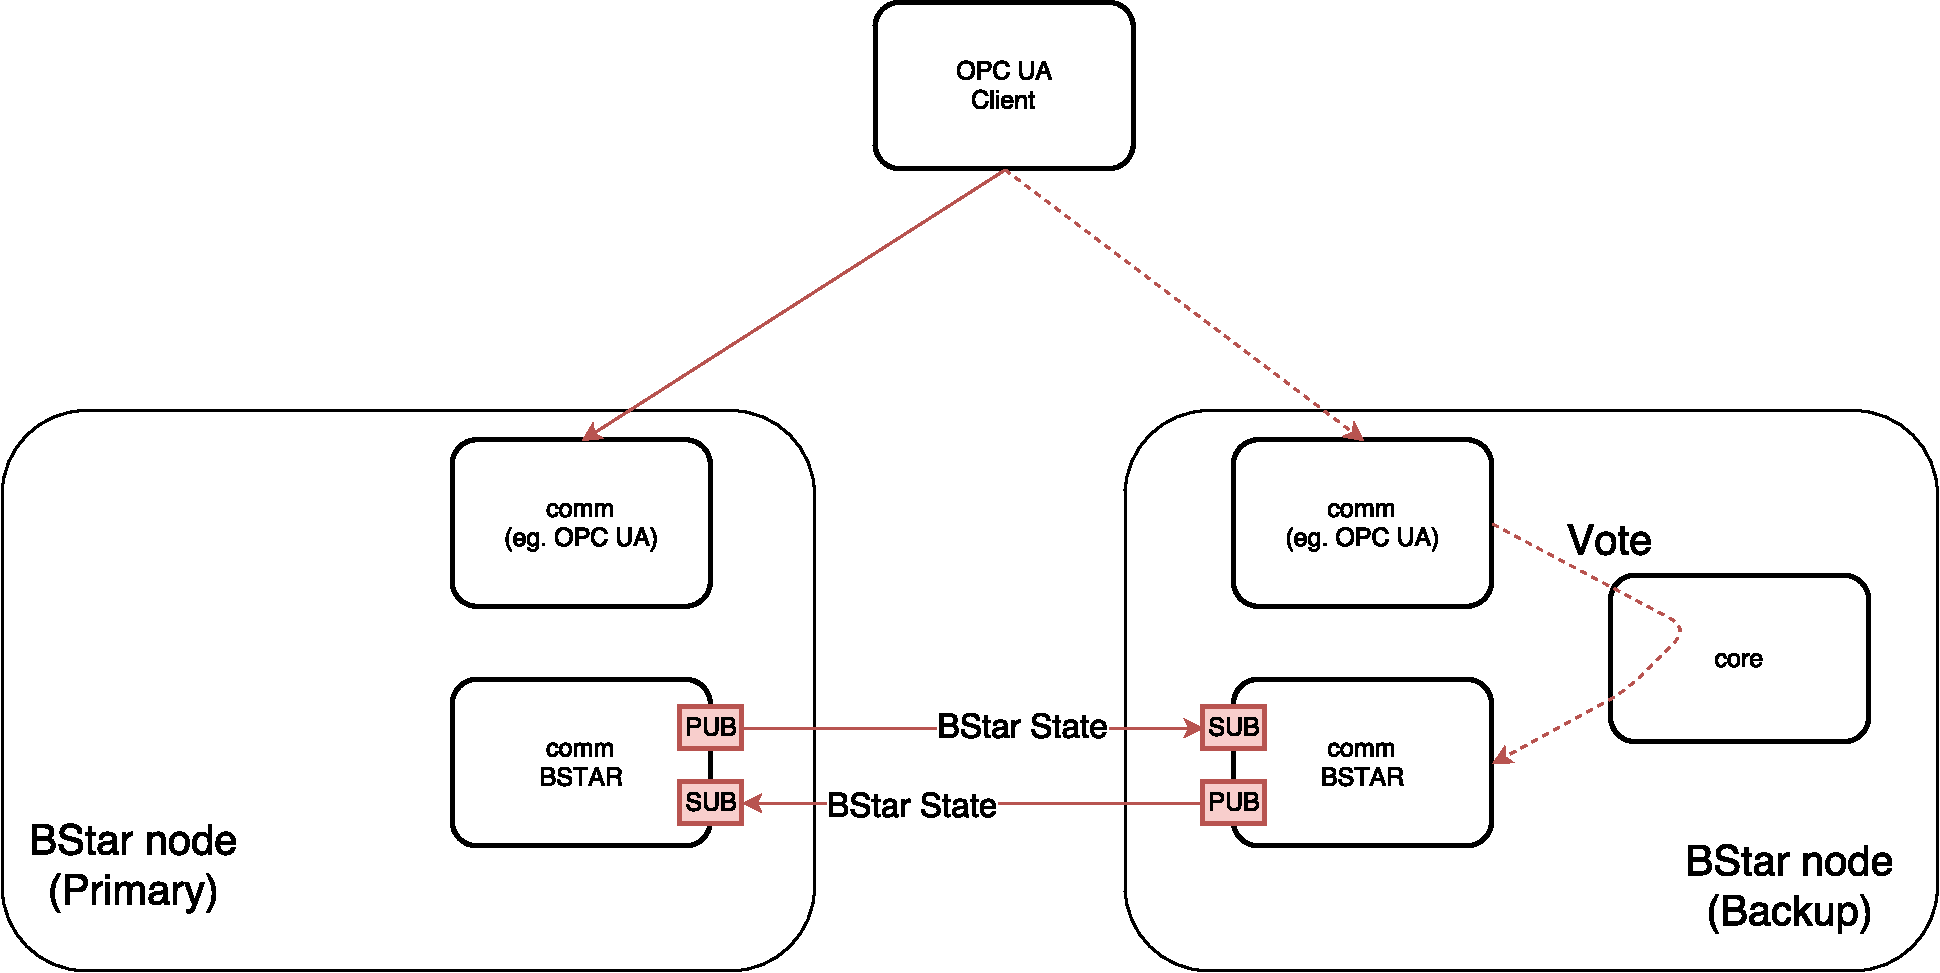
\includegraphics[width=\textwidth]{img/ML-HA_bstar.pdf}
	\caption{Schema of HA cluster and a higher level client}
	\label{fig:ml:ha}
\end{figure}

\subsubsection{Socket types}
The sockets used by both HA peers to send and receive heartbeats/state
information is a PUB-SUB pair each. This is useful to avoid queues filling up
in case of an actual failure. PUB sockets simply drop messages when there are
no SUB sockets connected, which is the desired effect.

\subsubsection{OPC UA}
One of the non-functional goals demanded the HA solution be developed with
\gls{opc-ua} in mind. OPC-UA describes several ways of non-transparent server
redundancy, which seems to map closely to how the \gls{bstar} works.

\subsection{Failover}
The passive node takes over when the following two conditions are met:

\begin{enumerate}
\item No life signs from the active node
\item Connection requests from clients
\end{enumerate}

The second condition is to prevent the split-brain syndrome and thus can be
thought of as an external vote for the node to actually initiate the failover.
This works because clients will try to (re-)connect to the HA peers in
round-robin fashion.  This algorithm is explained in \cite[Chapter 4 - Reliable
Request-Reply Patterns, Client-Side Reliability (Lazy Pirate
Pattern)]{zmq:zguide}.
% TODO: add Ruby example

In case the currently active peer crashes, the two conditions will be met.
This means that the passive node starts accepting snapshot requests (ICANHAZ
messages) and updates the DIM, so every other node will know about the new,
active node. This is needed for the message routing to work.

To establish or destroy connections (either to other nodes or to field
devices), callbacks from the \gls{bstar} library can be used to react on
becoming active and becoming passive. To do something in another actor,
Roadster's messaging infrastructure can be used.

% TODO Going active:
% * Core: guards (cases), ...
% * IoComm: peer connections
% * Downstream: subnode pinging, CSP publishing
% * Upstream: CSP pushing to supernode
% * Storage: ?
% * Logger: -


% TODO: Going passive
% TODO passive node: why not Ping subnodes too? Upstream sockets would have to be
%  connected to two nodes. => implement ROUTER-ROUTER


\subsubsection{No client, no failover}
A failover can only happen if there is at least one client. With no clients, a
vote cannot happen. Thinking about it, it is not a bad thing if the failover
cannot happen in that case, since there is no client depending on the service
brought by a HA cluster.

\subsubsection{Alarm generation}
% TODO using Guard
When a failover happens, it makes sense to create an alarm case in the
DIM, so the outage is visible to operational personnel in one of the web UIs.
The same applies to the case where the passive node goes down, although it
does not have an immediate effect on availability.  This is so the operational
personnel can act upon the alarm and e.g. initiate field forces to inspect the
failed node and repair it.

Once repaired, it is restarted with the exact same configuration --- either primary
or backup. Since there is already an active node (either the primary one,
or the backup one), the newly repaired node will become the new passive node.

\subsubsection{Failover from backup to primary node}
Once failed over, the newly actve backup node stays active. It does so until it
fails itself or is manually stopped. It never automatically switches back to
make the primary node the new active one without a failure. This is key. If a
node becomes unreachable, the failover happens automatically, but anything else will
require human interaction.

Subsequently, when the previously broken, primary node has been repaired, it
rejoins the \gls{bstar} cluster as the passive node. At that point, the backup
node can be killed if need be, and the primary node will take over again.  This
works because the \gls{bstar} operates symmetrically after a successful
handshake during initialization.

\subsection{Replication}
% diagonal HA
The passive HA peer needs to stay up-to-date, e.g. take part in DIM
synchronization. Instead of clients replicating modifications to both HA peers, as
described in \cite[Chapter 5 - Advanced Pub-Sub Patterns, The Clustered Hashmap
Protocol]{zmq:zguide}, the passive HA peer could just act as a supernode to the
active HA peer. This eliminates the need for an additional protocol. In case of
a failover, the roles of course need to be exchanged.

% TODO: what if HA cluster has supernode
{\color{red}A problem would be the case where the HA cluster has a supernode (although
considered an unusual case). That would mean the active peer has two supernodes
connected at the same time, which is not supported by the planned communication
infrastructure (especially with encryption, see
\autoref{sec:approach:encryption:ha}).  A solution could be to perform the
replication to the HA peer only via sockets of the two BSTAR actors.}

\subsection{Rolling upgrades}
% OPTIMIZE move to Discussion
An obvious side benefit of this comes into play with upgrades. Using the HA
cluster capability it is possible to perform rolling upgrades, meaning one HA
peer can be upgraded while the other one stays in service. After a successful
upgrade, Roadster on the active peer can be stopped, upgraded, and restarted as
the passive peer.

\subsection{A note on dedicated links}
The \gls{zguide} mentions that a dedicated network link between the two HA peers
(traditionally done with a crossover cable) is the best solution to prevent the
split-brain syndrome. This is true. But in some cases, it could also prevent a
failover from happening.

Imagine part of the currently active peer's network equipment fails, i.e. one
of its \glspl{NIC} connected to the switch fails, or one of its switch ports
fail. In that case it will be unreachable to the rest of the
federation or to the client. A failover would be desired. But it
cannot happen, since heartbeats will still be exchanged with the passive node over
the dedicated link. So it is a trade-off between risking the split-brain
syndrome and not being able to perform a failover.

\subsubsection{Extending the \gls{bstar}}\label{sec:approach:ha:bstar-ext}
% vision
Of course the \gls{bstar} mechanism could be extended to handle cases where the
active peer loses connectivity to its clients, but not to the other HA peer. In
a case like that, the passive node could actually take over to minimize
service downtime. The active HA peer could communicate the number of fully connected clients,
which would be zero in case it is cut off from its clients. That way, the
passive node could recognize the situation correctly, since it will get
requests from clients, which are trying to fallback to the passive peer since
the active peer is unresponsive. Knowing that the active peer has zero
connected clients, it could promote itself to the new active peer.

% what's needed for higher-level clients
For this to work, a way of counting fully connected (not just requesting)
clients has to be introduced. The COMM actor providing the \gls{opc-ua}
interface would know best how many clients are connected. This would solve the problem for single-level HA setups.

% what's needed for subnodes as clients
In case of a multi-level federation with a HA cluster at its root, the
cluster's subnodes form another set of clients. Because nodes within a
federation communicate with each other via \zmq sockets, telling how many
clients are connected is a bit less straight-forward, because \zmq abstracts
connection handling completely away. \zmq declares such needs as application matter.
The subnodes would have to implement application-level heartbeating.
That is, the subnodes that are fully connected at a given point in time (i.e. enrolled
in the DIM replication) would periodically send heartbeats which could then be
used to maintain an up-to-date list of active clients (where stale client
entries automatically expire).  The number of active clients (the size of the
list) could be communicated privately just between the two HA peers, along with
the heartbeats. Publishing that information via the DIM might be problematic,
since DIM updates go over the main network link.

% step down from active to passive
Something else needed is a HA peer's ability to step down from being the
active node as soon as its peer promotes itself to the newly active peer. In
the standard \gls{bstar} mechanism, this would be recognized as the split-brain
syndrome and handled fatally.

% discard because KISS
Doing this without an actual need would be a violation of the KISS principle,
so the first approach will not include any extensions to the \gls{bstar}.

\subsubsection{Corner case}
A highly unlikely, but dangerous corner case \emph{could} lead to the
split-brain syndrome. The following steps would be required to happen:

\begin{enumerate}
	\item the backup node is currently the active one

	\item then the dedicated link fails, which means no heartbeats are
		exchanged anymore

	\item a new client tries to connect or an existing one is temporarily
		gone and tries to reconnect
\end{enumerate}

Since clients most likely try to contact the primary node first, this could
lead to dreaded the split-brain syndrome. The primary node does not hear any
life signs from the backup node (the rightfully active peer), and client
requests count as votes. This means it will promote itself to the active peer,
even though the backup node is still active.

\subsection{A note on heart beating}\label{sec:approach:ha:hb}
Special attention needs to be paid when it comes to sending heartbeats within a
HA cluster. A na\"ive developer might implement the BSTAR actor so it
autonomously sends heartbeats. This works as long as the failures only affect
the hardware. But what if a software error happens in the CORE actor?  A
Roadster node certainly cannot function without the CORE actor. In that case the
BSTAR actor should not send out heartbeats anymore.

A better implementation would have the BSTAR actor periodically inquire (PING
request) the CORE actor whether it is still healthy, and only send out a
heartbeat in case it gets a response (PONG) in time. This can be done with a
simple mechanism, where the CORE actor is programmed to respond to every PING
request with a PONG response. Similar infrastructure of Roadster could be used
instead, if it already provides it.

Further ideas based on this fundamental mechanism are discussed in
\autoref{sec:discussion:imp:ha:hb}.

%----------------------------------------------------------------------------
\section{Persistence synchronization}\label{sec:approach:psync}
% TODO: big picture
The persisted data and updates to it, handled by the STORAGE actor, need to
bubble up and collected in the root node.

\subsection{Aspects}
There are multiple aspects involved in persistence synchronization:

\begin{description}
	\item [Initial synchronization:]\hfill\\
		How does one get the initial delta of updates since the last
		synchronization?


		\paragraph{Event journal} Event journal data is not
		append-only. Existing cases can still be modified, e.g. to
		confirm them. So the solution to get the full delta of
		modifications, but not more than needed, is to request the
		oldest non-finished case for each owning subnode (direct and
		indirect ones).

		\paragraph{Time series} The good thing about time series is
		that the records, once written, will not be modified. That allows
		for a very simple method of getting new time series records by
		just requesting all records added after a particular point in
		time, per series. However, since old time series data is
		deleted after a certain amount of time (e.g. 6 months), the
		timestamp of oldest record remaining also needs to be requested
		by the supernode, per series, so it can delete them from its
		local files as well.

		\paragraph{Parameters} Every param is owned by a node, and is
		synchronized through the DIM.  What is persisted is merely the
		last updated value so the node is able to boot with not only
		sensible defaults, but actual values that are most likely still
		correct. This means that there is no delta of modifications to
		communicate. Modifications to parameter objects in the DIM just
		need to be persisted.

	\item [Continuous synchronization:]\hfill\\
		Send further updates, one-by-one, in an event-driven manner.
		This is only needed in case the solution aims for event-driven
		(i.e. close to instantaneous) synchronization.

		\paragraph{Event journal} Non-finished cases live in the DIM.
		That means any node could theoretically persist a history of
		all cases owned by its subnodes (direct and indirect ones) by
		itself. Another way would be for any node to only create a
		persisted history its own cases and then communicate the
		modifications to the persisted data to its supernode. Every
		node would in turn include modifications from its subnodes
		(direct and indirect ones) in the stream of modifications to
		its supernode. {\color{red}It is not clear yet, what is the best
		solution here.}\\

		\paragraph{Time series} The most recent values of sensor data
		is held in the DIM. That means any node in the federation could
		do the sampling and persisting of time series data by itself.
		{\color{red}It is not clear yet what is the best solution here.}\\
		The deletion of old records does not have to be bubbled up,
		since that is done by a Roadster node autonomously whenever it
		persists a new one.

	\item [HA peer sync:]\hfill\\
		How is the passive HA peer updated?
		This not only matters when the supernode is a HA cluster (multi
		level), but also when it is at the bottom of the node hieararchy
		(single level).

		% diagnoal HA
		Same as with the DIM synchronization between HA peers, this
		could be done by simply treating the passive HA peer as a
		supernode.
\end{description}


\subsection{Variants}
There are multiple variants to achieve the needed functionality.

\subsubsection{Polling only}
The supernode just periodically request persistence
deltas. This would be handled over a DEALER-ROUTER pair of sockets. The nice
thing about this variant is that the subnode only has to do one thing, which is
responding to requests from the supernode(s); it does not have to proactively
send any updates after sending the an initial delta.

A big drawback is that the synchronization only happens periodically. This
does not seem to fit well into the overall Roadster architecture, which is
completely event-driven (no polls or "sleeps").

Another drawback is efficiency. This variant will periodically cause the
subnode's database to be searched for possibly large amounts of keys. Depending on the size of the
database and the efficiency of searching through keys, this could be a lot of
wasted resources or even cause bottle necks when interacting with the STOR
actor.

Overall, this variant is very simple, but does not offer some features we'd
normally expect from a framework like Roadster. The fruits are hanging low;
achieving event-driven synchronization and better efficiency is easy.

\subsubsection{Event-driven}
This variant avoids the delays introduced by the polling mechanism of the first
variant. Just like with the \gls{CSP}, the initial delta is requested and
communicated via the ROUTER-DEALER pair. As soon as the transmission of the
delta begins, the subnode also starts propagating any new modifications via the
PUSH socket. The supernode collects modifications from all subnodes through its
PULL socket.

To avoid filling the PUSH socket unnecessarily in case the supernode is
temporarily unavailable, the heartbeating done via the UPSTREAM/DOWNSTREAM actors will
be used to recognize such a situation. The continuous propagation of
modifications can be stopped, the sockets reinitialized, making the node ready
for whenever the supernode is back available.

\subsection{Chosen Variant}
No definite choice has been made yet. The client seems to favor the polling variant.
% TODO: choose a persistence synchronization variant

\section{Encryption}\label{sec:approach:encryption}
% TODO: big picture
It is fairly easy to enable transport security to secure the communication
between \zmq sockets over an unsecure network.

\subsection{Assigning socket roles}
Regarding the CURVE security mechanism in \zmq, one of the two involved sockets
needs to be designated as the CURVE server, and the other one as a CURVE
client.\footnote{This is a simple method call on each socket where the involved
keys are passed as well.} This will be done intuitively: A supernode's
DOWNSTREAM actor's sockets will act as CURVE servers, and a subnode's
UPSTREAM actor's sockets will act as CURVE clients. This is not just an
arbitrary choice: A CURVE client socket is given exactly one CURVE server
certificate. A supernode can have multiple subnodes, but the opposite is
impossible.\footnote{HA is a special case, see
\autoref{sec:approach:encryption:ha}} Thus, the socket inside the supernode's
DOWNSTREAM actor will be designated as the CURVE server, and the sockets
inside the subnodes' DOWNSTREAM actors will be designated as the CURVE
clients. An example of the client side is shown in \autoref{lst:auth:fednf}, as
performed by the UPSTREAM actor.

\begin{listing}
	\inputminted[bgcolor=bg]{Ruby}{listings/auth/fednf.rb}
	\caption{Enabling CURVE mechanism on the client}
	\label{lst:auth:fednf}
\end{listing}

\subsection{Mutual authentication}
% keys on both sides, and which nodes need whose public key
In addition to the server authentication, which is always performed, client
side authentification is desired. This means that each federation node must be
in possession of its respective clients' public keys.

% distribution of public keys
Public keys and the private keys are generated in pairs.  Due to
the nature of public keys, they can be distributed conveniently and safely
through the shared configuration file that defines the federation
topology.\footnote{Curve25519 public keys are only 40 ASCII characters long in
\gls{Z85} notation.}

% distribution of secret keys via SSH
However, distributing the private keys is less convenient, since they must be kept
private. This can be done via \gls{SSH}, logging into each node and generating
the key pair right on the node itself. This way, the private keys would never
even touch the network.

\subsubsection{ZAP}
A socket designated as CURVE server needs a way to authenticate arriving client
connections. This is done via an in-process \gls{ZAP} authentication handler,
as described in \autoref{sec:zmq:security}. That authentication handler
needs to be able to access all clients' public keys to be able to perform its
job.

The ZAP protocol (used between a CURVE server socket and the authentication
handler) is very simple and thus makes it possible to relay the authentication
requests from there to a central ZAP authentication handler, so all clients'
public keys could be stored and managed centrally. But that would violate the
autonomy requirement, so this idea has been discarded immediately.

CZMQ provides an authentication handler\footnote{It is simply a function
(\cpp{zauth()}) that is executed by a CZMQ actor. The whole construct is
abstracted in CZTop through \rb{CZTop::Authenticator}.} that can lookup public
keys awaiting authentication in a designated directory on the file system,
which it does by instantiating a certificate store.\footnote{That certificate
store is a class in CZMQ called \cpp{zcertstore}, represented through
\rb{CZTop::CertStore} in CZTop.} The certificate store in turn looks up the
certificates on disk by the public key in question.

There is also the possibility of providing an already instanciated certificate
store to the authentication handler. This is useful because a certificate store
allows the insertion of certificates (public keys) in-memory, avoiding the need
to load certificates from disk. This greatly simplifies the key distribution.
Public key files will not have to be copied from one node to its subnodes
anymore. Instead, they can be taken directly from the shared configuration file
that defines the federation topology. As an example, \autoref{lst:auth:fedsf}
shows how to start an authentication handler which does client authentication
as it is done inside the DOWNSTREAM actor.

\begin{listing}
	\inputminted[bgcolor=bg]{Ruby}{listings/auth/fedsf.rb}
	\caption{Enabling CURVE mechanism on the server to perform client authentication}
	\label{lst:auth:fedsf}
\end{listing}

\paragraph{Failover}\label{sec:approach:encryption:ha}
It is possible that a node's supernode is actually a HA cluster consisting of
two nodes. Those two nodes should have their own key pairs for additional
security. This imposes a problem for the subnodes: It is only possible to assign
a single CURVE server certificate (public key). In case the active HA peer becomes
unresponsive and the subnode(s) falls back to the passive HA peer, a new CURVE
server certificate needs to be assigned to the client sockets. This should be
possible. But there's a better solution:
Since the socket could be \cite[Binary Star Implementation, Binary Star client
in C]{zmq:zguide} ``confused''\footnote{This probably applies only to REQ
sockets, since they implement \cite[Client-Side Reliability (Lazy Pirate
Pattern)]{zmq:zguide} ``a small finite-state machine to enforce the
send/receive ping-pong''}, it is good practice to simply destroy the existing
socket and create a fresh one, assigning the correct supernode's CURVE server
certificate to it.

\paragraph{IP based access control}
In addition to the CURVE mechanism, blacklisting or whitelisting clients based
on their \gls{IP} addresses is possible and supported by
\rb{CZTop::Authenticator} through the PLAIN mechanism. It would even be
feasible to whitelist the exact client IP addresses, since they can be deduced
from the shared configuration. But it is not part of requirements and thus will not
be done within the scope of this bachelor thesis.

\subsection{Key generation and distribution procedure}
The following procedure can be followed to generate the required keys in
advance and make them available through the shared configuration file:

\begin{enumerate}
	\item for all nodes
	\begin{enumerate}
		\item generate key pair on the node itself and save it on the
			node
		\item remember the public key
	\end{enumerate}

	\item put all public keys (in Z85 notation) to their respective section
		in the shared config file defining the federation topology
\end{enumerate}

This procedure could be implemented as a script that performs the procedure
over \gls{SSH} while the nodes are still in the
lab (assuming that is secure). Of course that script could also be used when
the nodes are already installed in a production environment. However, for that to be
secure, the nodes' authenticities must have been established in advance, or
man-in-the-middle attacks would be possible while logging into the nodes,
compromising everything.

% TODO: `roadster keygen CONFIG` util

% TODO 256 bit encryption
% TODO 16 byte authenticator
% TODO 24 byte nonce

% TODO Entropy without encryption:
% ```
% Entropy = 5.390141 bits per byte.
% 
% Optimum compression would reduce the size
% of this 4518 byte file by 32 percent.
% 
% Chi square distribution for 4518 samples is 36298.08, and randomly
% would exceed this value less than 0.01 percent of the times.
% 
% Arithmetic mean value of data bytes is 83.2517 (127.5 = random).
% Monte Carlo value for Pi is 4.000000000 (error 27.32 percent).
% Serial correlation coefficient is 0.310227 (totally uncorrelated = 0.0).
% ```

\section{OPC UA Interface: High availability}\label{sec:approach:opc-ua}
The OPC UA standard seems pretty complicated. And given that the requirement
is not concrete yet, no possible solution has been worked out yet.

In case it is non-transparent server redundancy, \cite[6.4.2.4 Non-transparent
Redundancy, p.~96]{opc-ua:behavior:server-redundancy} describes the exact
behavior.

% TODO study standard
% TODO use Andy's gem (it "should be a simple thing")
